% AA-28 | Iteracja XIV; szczegółowy audyt historyczny III, 20 XI 2026.
\chapter{Ciała cyklotomiczne i wielomiany cyklotomiczne}
\label{aa:ch:cyclotomic}
\section{Pierwiastki pierwotne i wielomiany cyklotomiczne}

W teorii Galois ważnym źródłem rozszerzeń abelowych są ciała
otrzymywane przez dołączenie pierwiastków z jedynki.
Zamiast rozpoczynać od wzorów z funkcją wykładniczą zespoloną,
rozważymy czysto algebraicznie pierwiastki równania $X^n=1$.
To podejście nie wymaga analitycznej konstrukcji $\mathbb R$
ani definicji funkcji wykładniczej. Jeżeli zechcemy narysować
pierwiastki w płaszczyźnie zespolonej, skorzystamy jedynie
z geometrycznej interpretacji $\mathbb C$, traktowanego tutaj
jako uprzednio dane ciało, zob. rozdział~\ref{aa:ch:fields-fractions}.

\begin{definicja}\label{aa:def:cyclotomic}
Niech $n\ge1$ będzie liczbą całkowitą. W ustalonym domknięciu
algebraicznym $\overline{\mathbb Q}$ wybieramy element
$\zeta_n$ o \emph{dokładnym rzędzie multiplikatywnym $n$}:
$\zeta_n^n=1$ oraz $\zeta_n^d\ne1$ dla każdej liczby
całkowitej $1\le d<n$. Taki element nazywamy
\emph{pierwotnym $n$-tym pierwiastkiem z jedynki}.
Przyjmujemy $\zeta_1=1$. Definiujemy
\[
\Phi_n(X)=\prod_{\substack{1\le k\le n\\\gcd(k,n)=1}}
(X-\zeta_n^k)\in\overline{\mathbb Q}[X].
\]
Jest to \emph{$n$-ty wielomian cyklotomiczny}. Symbol
$\varphi(n)$ oznacza liczbę liczb całkowitych
$1\le k\le n$ względnie pierwszych z $n$.
\end{definicja}

\begin{uwaga}[Istnienie i niezależność od wyboru pierwiastka]
W charakterystyce $0$ pochodna $X^n-1$ ma postać
$nX^{n-1}$ i jest względnie pierwsza z $X^n-1$.
W $\overline{\mathbb Q}$ wielomian $X^n-1$ ma więc
$n$ różnych pierwiastków. Stanowią one skończoną podgrupę
multiplikatywną ciała, a każda skończona podgrupa grupy
multiplikatywnej ciała jest cykliczna (zob. wyniki
z rozdziału~\ref{aa:ch:kummer}).
Istnieje zatem jej generator rzędu $n$.
Jeśli $\eta_n$ jest innym generatorem, to
$\eta_n=\zeta_n^u$ z $\gcd(u,n)=1$.
Mnożenie przez $u$ permutuje klasy liczb względnie
pierwszych z $n$, dlatego zbiór czynników w definicji
$\Phi_n$ nie zależy od wyboru $\zeta_n$.
Dla $n=1$ definicja daje $\Phi_1(X)=X-1$.
\end{uwaga}

\begin{twierdzenie}[Rozkład wielomianu $X^n-1$]
\label{aa:tw:cyclotomic-product}
Dla każdej liczby całkowitej $n\ge1$ zachodzi równość
\[
X^n-1=\prod_{d\mid n}\Phi_d(X)
\qquad\text{w }\mathbb Z[X].
\]
Ponadto każdy $\Phi_n$ jest moniczny, należy do $\mathbb Z[X]$
i ma stopień $\varphi(n)$.
\end{twierdzenie}
\begin{proof}
\emph{Krok 1: rozkład według rzędów.} Pierwiastki
$X^n-1$ są różne. Rząd $d$ dowolnego takiego pierwiastka
dzieli $n$. Z kolei każdy pierwiastek dokładnego rzędu
$d\mid n$ jest pierwiastkiem $X^n-1$. Zbiory pierwiastków
poszczególnych dokładnych rzędów są rozłączne, a zbiór
pierwiastków rzędu $d$ ma $\varphi(d)$ elementów:
przy ustalonym generatorze są to dokładnie
$\zeta_d^k$ z $\gcd(k,d)=1$. Ponieważ obie strony są
wielomianami monicznymi i mają te same pierwiastki
z krotnościami $1$, otrzymujemy tożsamość w
$\overline{\mathbb Q}[X]$. Z definicji wynika też
$\deg\Phi_n=\varphi(n)$.

\emph{Krok 2: całkowitość współczynników.}
Przeprowadzimy indukcję po $n$. Dla $n=1$ mamy
$\Phi_1=X-1\in\mathbb Z[X]$. Niech $n>1$ i załóżmy,
że $\Phi_d\in\mathbb Z[X]$ dla wszystkich $d<n$.
Wówczas
\(Q(X)=\prod_{d\mid n,\,d<n}\Phi_d(X)\)
jest monicznym wielomianem w $\mathbb Z[X]$.
Algorytm dzielenia przez moniczny wielomian działa nad
\emph{dowolnym} pierścieniem współczynników: odejmujemy
kolejne wielokrotności $Q$, aby usuwać najwyższe wyrazy.
Otrzymujemy więc $H,R\in\mathbb Z[X]$ takie, że
$X^n-1=QH+R$ i $R=0$ albo $\deg R<\deg Q$.
Jednocześnie krok pierwszy daje $X^n-1=Q\Phi_n$
w $\overline{\mathbb Q}[X]$. Jednoznaczność dzielenia
w tym ciele implikuje $R=0$ i $H=\Phi_n$. Stąd
$\Phi_n\in\mathbb Z[X]$ i jest moniczny.
\end{proof}

Aby dowieść nierozkładalności $\Phi_n$ nad $\mathbb Q$,
nie wystarczy znać jego pierwiastki. Trzeba wykazać, że
minimalny wielomian jednego pierwiastka zawiera również
wszystkie pozostałe pierwiastki pierwotne. Kluczowy jest
poniższy argument z redukcją modulo liczbę pierwszą.

\begin{lemat}[Zamiana pierwiastka przez potęgę pierwszą]
\label{aa:lem:cyclotomic-prime}
Niech $n\ge1$, $\alpha\in\overline{\mathbb Q}$ będzie
pierwotnym $n$-tym pierwiastkiem z jedynki, zaś
$f\in\mathbb Z[X]$ jego monicznym wielomianem minimalnym
nad $\mathbb Q$. Jeżeli $\ell$ jest liczbą pierwszą
względnie pierwszą z $n$, to $f(\alpha^\ell)=0$.
\end{lemat}
\begin{proof}
Załóżmy przeciwnie, że $f(\alpha^\ell)\ne0$.
Ponieważ $\gcd(\ell,n)=1$, element $\alpha^\ell$
ma dokładny rząd $n$. Niech $g\in\mathbb Z[X]$ będzie
jego monicznym wielomianem minimalnym nad $\mathbb Q$.
Jego współczynniki są całkowite: $\alpha^\ell$ jest
pierwiastkiem monicznego $\Phi_n\in\mathbb Z[X]$, a
moniczny czynnik nierozkładalny takiego wielomianu ma
współczynniki w $\mathbb Z$ na mocy lematu Gaussa.
Wielomiany $f$ i $g$ są różne, ponieważ
$f(\alpha^\ell)\ne0$, i oba dzielą $X^n-1$ w
$\mathbb Z[X]$. Są nierozkładalne nad $\mathbb Q$, a więc
względnie pierwsze w $\mathbb Q[X]$. Ich iloczyn
$fg$ dzieli $X^n-1$ w $\mathbb Z[X]$:
najpierw uzyskujemy tę podzielność w $\mathbb Q[X]$,
a następnie stosujemy lemat Gaussa do wielomianów monicznych.

Ponieważ $g(\alpha^\ell)=0$, mamy
$(g(X^\ell))(\alpha)=0$. Minimalność $f$ daje
$f\mid g(X^\ell)$ w $\mathbb Q[X]$ i, ponownie z
moniczności i lematu Gaussa, w $\mathbb Z[X]$.
Oznaczmy redukcję współczynników modulo $\ell$ kreską.
W charakterystyce $\ell$ zachodzi
$\overline{g(X^\ell)}=\overline g(X)^\ell$, toteż
\(\overline f\mid\overline g(X)^\ell\)
w $\mathbb F_\ell[X]$. Wielomian $\overline f$ jest
niezerowy i moniczny. Wybierzmy dowolny jego moniczny
nierozkładalny dzielnik $h$. Ponieważ $h$ jest
pierwszy w pierścieniu $\mathbb F_\ell[X]$, z
$h\mid\overline g^\ell$ wynika $h\mid\overline g$.
Oznacza to, że $h^2$ dzieli
$\overline f\,\overline g=\overline{fg}$, a zatem
$\overline{X^n-1}$. Jest to niemożliwe, ponieważ
$\ell\nmid n$ i
\[
\gcd(X^n-1,\,nX^{n-1})=1
\quad\text{w }\mathbb F_\ell[X].
\]
Rzeczywiście, wielomian $X^n-1$ nie ma wspólnego
pierwiastka z $X^{n-1}$, a $n$ jest niezerowym skalarem
w $\mathbb F_\ell$. Zatem $X^n-1$ jest bez czynników
powtórzonych, w sprzeczności z podzielnością przez $h^2$.
\end{proof}

\begin{twierdzenie}[Nierozkładalność wielomianów cyklotomicznych]
\label{aa:tw:cyclotomic-irreducible}
Dla każdej liczby całkowitej $n\ge1$ wielomian
$\Phi_n\in\mathbb Z[X]$ jest nierozkładalny nad
$\mathbb Q$.
\end{twierdzenie}
\begin{proof}
Dla $n=1$ otrzymujemy wielomian liniowy $X-1$.
Niech $n>1$ i niech $\alpha$ będzie pierwotnym
$n$-tym pierwiastkiem z jedynki. Oznaczmy przez $f$
jego moniczny wielomian minimalny nad $\mathbb Q$.
Wielomian $f$ dzieli $\Phi_n$, a jego współczynniki
należą do $\mathbb Z$ na mocy lematu Gaussa.

Weźmy dowolną liczbę całkowitą $k\ge1$ z
$\gcd(k,n)=1$. Jeżeli $k=1$, to $f(\alpha^k)=0$
z definicji. Gdy $k>1$, rozłóżmy $k$ na iloczyn liczb
pierwszych $k=\ell_1\cdots\ell_r$. Każda $\ell_j$
jest względnie pierwsza z $n$. Stosujemy kolejno
Lemat~\ref{aa:lem:cyclotomic-prime}: najpierw
$f(\alpha^{\ell_1})=0$, następnie
$f(\alpha^{\ell_1\ell_2})=0$ i tak dalej.
Na każdym etapie aktualny pierwiastek ma nadal
rząd $n$, a ponieważ jest pierwiastkiem nierozkładalnego
$f$, jego wielomianem minimalnym także jest $f$;
wszystkie warunki lematu pozostają zatem spełnione.
Otrzymujemy $f(\alpha^k)=0$.

W ten sposób $f$ ma wszystkie $\varphi(n)$ parami
różne pierwiastki $\Phi_n$. Ponieważ $f$ i $\Phi_n$
są moniczne, a $f\mid\Phi_n$, wynika $f=\Phi_n$.
\end{proof}

\section{Grupa Galois i przykłady}

\begin{twierdzenie}[Grupa Galois ciała cyklotomicznego]
\label{aa:tw:cyclotomic-galois}
Dla każdej liczby całkowitej $n\ge1$ rozszerzenie
$\mathbb Q(\zeta_n)/\mathbb Q$ jest Galois stopnia
$\varphi(n)$, a przyporządkowanie
\[
\sigma\longmapsto [k]_n\quad\text{gdzie}\quad
\sigma(\zeta_n)=\zeta_n^k
\]
wyznacza izomorfizm
\(\operatorname{Gal}(\mathbb Q(\zeta_n)/\mathbb Q)
\cong(\mathbb Z/n\mathbb Z)^\times\).
Dla $n=1$ obie grupy są trywialne.
\end{twierdzenie}
\begin{proof}
Z Twierdzenia~\ref{aa:tw:cyclotomic-irreducible} mamy
$[\mathbb Q(\zeta_n):\mathbb Q]=\deg\Phi_n=\varphi(n)$.
Wielomian $\Phi_n$ ma różne pierwiastki, gdyż dzieli
$X^n-1$ w charakterystyce zero. Wszystkie jego
pierwiastki są postaci $\zeta_n^k$ i należą do
$\mathbb Q(\zeta_n)$, więc jest to ciało rozkładu
wielomianu rozdzielczego; rozszerzenie jest Galois.

Niech $\sigma$ będzie automorfizmem tego rozszerzenia.
Ponieważ $\Phi_n(\sigma(\zeta_n))=0$,
istnieje $k$, względnie pierwszy z $n$, taki że
$\sigma(\zeta_n)=\zeta_n^k$. Klasa $[k]_n$ jest
jednoznacznie wyznaczona, bo $\zeta_n$ ma rząd $n$.
Jeżeli dwa automorfizmy mają ten sam obraz $\zeta_n$,
to zgadzają się na generatorze i na $\mathbb Q$, a
więc są równe. Odwzorowanie z tezy jest więc iniektywne.
Dla każdego $[k]_n\in(\mathbb Z/n\mathbb Z)^\times$
element $\zeta_n^k$ jest pierwiastkiem tego samego
nierozkładalnego wielomianu minimalnego $\Phi_n$.
Istnieje zatem $\mathbb Q$-zanurzenie
$\mathbb Q(\zeta_n)\to\mathbb Q(\zeta_n)$
wysyłające $\zeta_n$ na $\zeta_n^k$. Jego obraz jest
całym ciałem, gdyż $k$ jest odwracalny modulo $n$:
$\zeta_n=(\zeta_n^k)^u$ dla odpowiedniego $u$.
Jest to więc automorfizm, co dowodzi surjektywności.
Jeśli $\sigma(\zeta_n)=\zeta_n^k$ oraz
$\tau(\zeta_n)=\zeta_n^\ell$, to
$(\sigma\circ\tau)(\zeta_n)=\zeta_n^{k\ell}$.
Mnożenie klas jest zatem zgodne ze składaniem
automorfizmów, co kończy dowód.
\end{proof}

\begin{figure}[htbp]
\centering
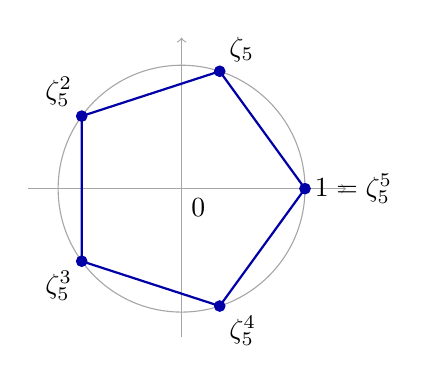
\begin{tikzpicture}[scale=0.95]
  \draw[gray!70] (0,0) circle (1.65);
  \draw[->,gray!70] (-2.05,0)--(2.2,0);
  \draw[->,gray!70] (0,-1.98)--(0,2.02);
  \draw[blue!65!black,thick] (0:1.65)--(72:1.65)--(144:1.65)--(216:1.65)--(288:1.65)--cycle;
  \foreach \k in {0,...,4} {\filldraw[blue!65!black] (72*\k:1.65) circle (2pt);}
  \node[right] at (0:1.65) {$1=\zeta_5^5$};
  \node[above right] at (72:1.65) {$\zeta_5$};
  \node[above left] at (144:1.65) {$\zeta_5^2$};
  \node[below left] at (216:1.65) {$\zeta_5^3$};
  \node[below right] at (288:1.65) {$\zeta_5^4$};
  \node[below right] at (0,0) {$0$};
\end{tikzpicture}
\caption{Pięć pierwiastków równania $X^5=1$ na okręgu jednostkowym
w płaszczyźnie zespolonej. Cztery pierwiastki różne od $1$ są
sprzężone nad $\mathbb Q$ i są pierwiastkami $\Phi_5$.}
\label{aa:fig:cyclotomic-five}
\end{figure}

\begin{przyklad}[Ciało piątych pierwiastków z jedynki]
\label{aa:prz:cyclotomic-five}
Dla $n=5$, ponieważ jedynymi dodatnimi dzielnikami $5$
są $1$ i $5$, z Twierdzenia~\ref{aa:tw:cyclotomic-product}
wynika
\[
\Phi_5(X)=\frac{X^5-1}{X-1}
=X^4+X^3+X^2+X+1.
\]
Element $2\bmod5$ generuje grupę
$(\mathbb Z/5\mathbb Z)^\times$, gdyż jego kolejne
potęgi modulo $5$ to $2,4,3,1$.
Stąd $\operatorname{Gal}(\mathbb Q(\zeta_5)/\mathbb Q)$
jest cykliczna rzędu $4$.
Jej jedyna podgrupa rzędu $2$ to
$H=\{\sigma_1,\sigma_{-1}\}$, gdzie
$\sigma_{-1}(\zeta_5)=\zeta_5^{-1}$; przy zespolonej
realizacji jest to sprzężenie zespolone.

Połóżmy $u=\zeta_5+\zeta_5^{-1}$. Jest on stały pod
$H$. Z równania
$1+\zeta_5+\zeta_5^2+\zeta_5^3+\zeta_5^4=0$
po podzieleniu przez $\zeta_5^2$ otrzymujemy
$1+(\zeta_5+\zeta_5^{-1})
 +(\zeta_5^2+\zeta_5^{-2})=0$.
Ponieważ
$\zeta_5^2+\zeta_5^{-2}=u^2-2$,
odpowiednia równość ma postać
$u^2+u-1=0$. Wyróżnik tego wielomianu jest równy $5$,
które nie jest kwadratem liczby wymiernej; zatem
$[\mathbb Q(u):\mathbb Q]=2$.
Z odpowiedniości Galois wynika, że ciało elementów stałych $E^H$
również ma stopień $4/2=2$ nad $\mathbb Q$.
Ponieważ $\mathbb Q(u)\subseteq E^H$ i obie strony mają
stopień $2$, otrzymujemy
$E^H=\mathbb Q(\zeta_5+\zeta_5^{-1})$.
Rysunek~\ref{aa:fig:cyclotomic-five} pokazuje położenie
pierwiastków, ale obliczenie stopni i ciała stałego jest
czysto algebraiczne.
\end{przyklad}

\begin{przyklad}[Grupa Galois nie musi być cykliczna]
\label{aa:prz:cyclotomic-eight}
Dla $n=8$ pierwiastki rzędu dokładnie $8$ spełniają
$X^4=-1$, a zatem $\Phi_8(X)=X^4+1$. Rzeczywiście,
wszystkie cztery pierwiastki $X^4+1$ są pierwiastkami
$X^8-1$, lecz nie $X^4-1$, więc mają dokładny rząd $8$.
Grupa
$(\mathbb Z/8\mathbb Z)^\times=\{[1],[3],[5],[7]\}$
ma cztery elementy, przy czym
$3^2\equiv5^2\equiv7^2\equiv1\pmod8$.
Nie jest więc cykliczna rzędu $4$ (nie ma elementu
rzędu $4$), lecz jest izomorficzna z $C_2\times C_2$.
To kontrprzykład dla stwierdzenia, że każda grupa
Galois ciała cyklotomicznego jest cykliczna.
\end{przyklad}

\begin{uwaga}[Charakterystyka dodatnia]
\label{aa:uw:cyclotomic-characteristic}
Dowód nierozkładalności $\Phi_n$ dotyczył ciała
$\mathbb Q$. Nie wolno bez dodatkowych założeń twierdzić,
że redukcja $\Phi_n$ modulo liczbę pierwszą $p$ pozostaje
nierozkładalna albo rozdzielcza. Na przykład
\[
\Phi_3(X)=X^2+X+1=(X-1)^2
\qquad\text{w }\mathbb F_3[X].
\]
Równość wynika z rozwinięcia $(X-1)^2=X^2-2X+1$
i kongruencji $-2\equiv1\pmod3$.
Pochodna $X^n-1$ w charakterystyce $p$ jest
$nX^{n-1}$; rozdzielczość jest zapewniona dokładnie
wtedy, gdy $p\nmid n$. Nawet w tym przypadku
nierozkładalność $\Phi_n$ nad $\mathbb Q$ sama w sobie
nie implikuje nierozkładalności po redukcji.
\end{uwaga}
